\documentclass[
%11pt, % The default document font size, options: 10pt, 11pt, 12pt
%oneside, % Two side (alternating margins) for binding by default, uncomment to switch to one side
english, % ngerman for German
%singlespacing, % Single line spacing, alternatives: onehalfspacing or doublespacing
%draft, % Uncomment to enable draft mode (no pictures, no links, overfull hboxes indicated)
%nolistspacing, % If the document is onehalfspacing or doublespacing, uncomment this to set spacing in lists to single
%liststotoc, % Uncomment to add the list of figures/tables/etc to the table of contents
%toctotoc, % Uncomment to add the main table of contents to the table of contents
%parskip, % Uncomment to add space between paragraphs
%nohyperref, % Uncomment to not load the hyperref package
headsepline, % Uncomment to get a line under the header
%chapterinoneline, % Uncomment to place the chapter title next to the number on one line
%consistentlayout, % Uncomment to change the layout of the declaration, abstract and acknowledgements pages to match the default layout
]{article} % The class file specifying the document structure

\usepackage[utf8]{inputenc} % Required for inputting international characters
\usepackage{hyperref} % Working URL links
\usepackage[toc,page]{appendix} % Table of contents, etc.

\usepackage{graphicx, graphbox, subcaption} % Images
\graphicspath{ {./images/} }

\usepackage{listings}
\usepackage{color}
    \lstloadlanguages{C,[Sharp]C,C++,csh,Java, Python}
    
    \definecolor{bluekeywords}{rgb}{0.13,0.13,1}
    \definecolor{greencomments}{rgb}{0,0.5,0}
    \definecolor{redstrings}{rgb}{0.9,0,0}

    \lstset{
    language=python,
    showspaces=false,
    showtabs=false,
    numbers=left,
    stepnumber=1,
    showstringspaces=false,
    tabsize=1,
    breaklines=true,
    breakatwhitespace=true,
    escapeinside={(*@}{@*)},
    commentstyle=\color{greencomments},
    keywordstyle=\color{bluekeywords}\bfseries,
    stringstyle=\color{redstrings},
    basicstyle=\ttfamily,
    }

\usepackage{biblatex}
\addbibresource{biblio}
\usepackage{csquotes}

\usepackage{siunitx, booktabs}

\usepackage{todonotes}

\begin{document}
\begin{center}
    \Large 
        \textbf{Minimax and Alpha/Beta Pruning for Tic-Tac-Toe}\\
    \normalsize

    Frederik Blem - cph-fb114@cphbusiness.dk\\
    Simon Schønberg Bojesen - cph-sb339@cphbusiness.dk\\

    \large
        Copenhagen Business Academy\\
        Supervisor: Martin Vestergaard\\
        %Examiner: Mr. Exam Miner
    \normalsize
\end{center}
\thispagestyle{empty}
\textbf{Abstract}
\begin{abstract}
    \label{sec:abstract}
    The problem with the Minimax algorithm is that it spends too much time evaluating moves that are worse than already considered moves.
    %say why it is interesting
    It is interesting to resolve this for improving the performance of games with many possible moves.
    %say what your solution achieves
    This solution presents an implementation of Alpha Beta Pruning which drastically reduced the amount of considered moves in the Minimax algorithm.
    %say what follows from your solution
    From the solution the conclusion is that Alpha Beta Pruning could significantly improve performance in games that require many moves to win.
\end{abstract} 
%\clearpage
\tableofcontents % Prints the main table of contents
%\listoffigures % Prints the list of figures
%\listoftables % Prints the list of tables
\clearpage
\pagenumbering{arabic}
\input{sections/Introduction.tex}

\section{Minimax Algorithm} 
\label{sec:Minimax Algorithm}

\subsection{Introduction to Minimax}
\label{subsec:Introduction to Minimax}
The Minimax algorithm is a recursive algorithm which is used in turn-based games like chess and tic-tac-toe, 
to make the AI player consider all possible moves and choose the most rational one.

\subsection{Explanation of Minimax}
\label{subsec:Explanation of Minimax}
\subsubsection{About Minimax}
First, it is important to understand the meaning behind recursive code. 
When code is recursive, it for example means that it's a function that calls itself with updated arguments until it reaches some condition the function wants to return. 
In the Minimax algorithm, the function is made to call itself in order to keep looking at more possible future moves, 
and ultimately decides which move is the best move to make on the AI’s current board.
\subsubsection{Why is it called Minimax}
The idea behind minimax is that the algorithm expects the game to be a turn-based 2-player game, and the algorithm defines these 2 players as the minimizer and the maximizer. 
This simply means that the algorithm always expects the minimizer to pick the move with the lowest score, and the maximizer to do the opposite. 
Here is an example: Here the maximizer is the human player and the minimizer is the AI player in this scenario.\\

\begin{figure}
    \caption{An example of a Tic-Tac-Toe board}
    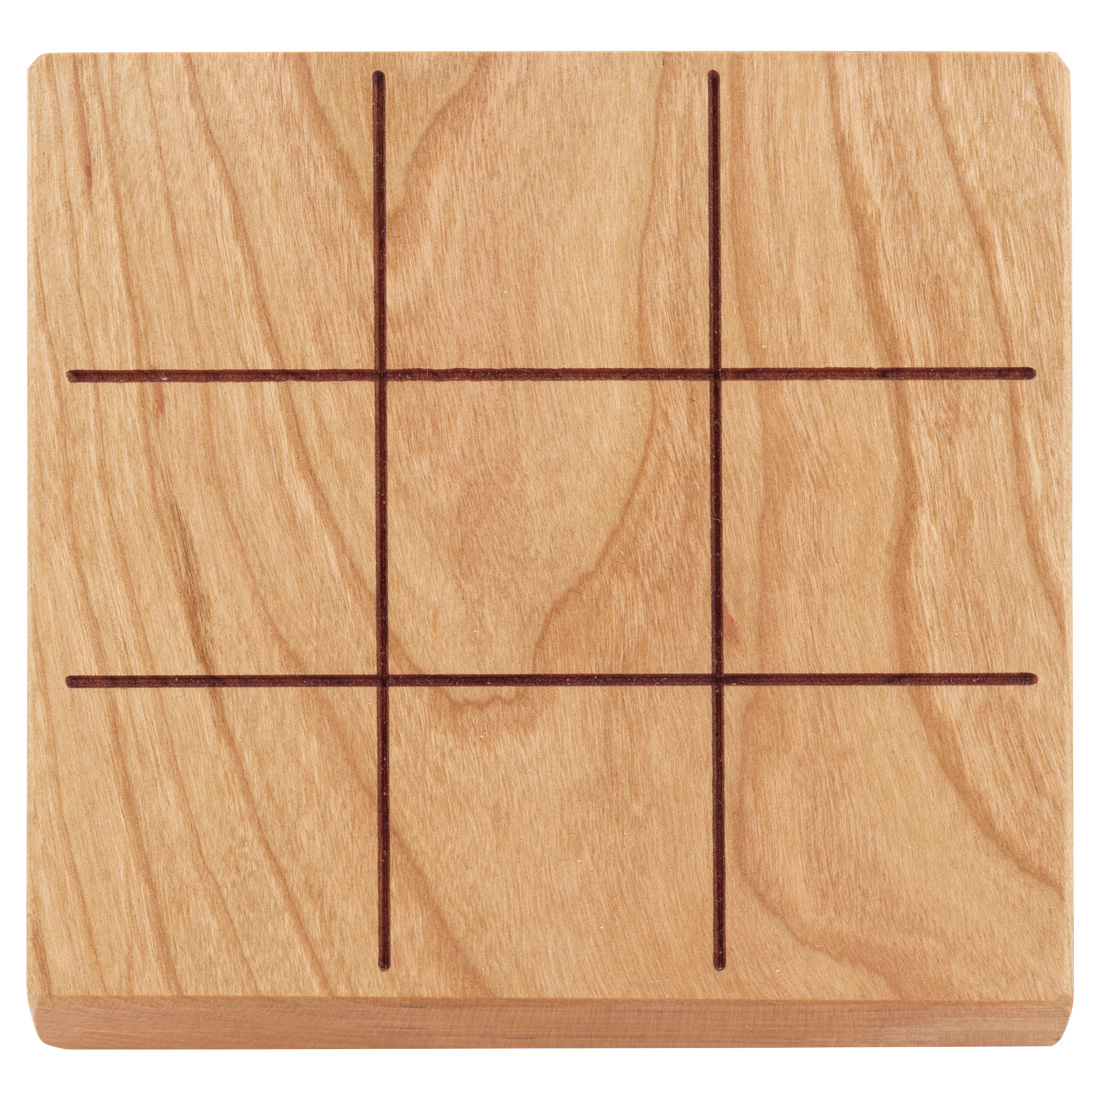
\includegraphics[width=\textwidth]{89-137-4480.jpg}
    \label{fig:Board Example}
\end{figure}

Consider the Tic-Tac-Toe board in figure~\ref{fig:Board Example}.\\


In this scenario the AI player goes first as “X” and tries to figure out the most rational move of the 9 moves possible. 
It does this by predicting what the opposing player, maximizer would then do on his next move and so on until it has found the fastest way to win for that one move. 
Basically, the algorithm runs a simulated game on each of the current board’s possible moves, against the maximizer, 
and when it is done with one move it backtracks back to the current board with that moves score value, to run a new simulation on the next move. 
When it has simulated how to win by all the possible moves it will then make the move that will help it win the fastest.\\

Consider again another example in figure~\ref{fig:Tree Example}.\\
\begin{figure}
    \caption{Minimax Tree Example}
    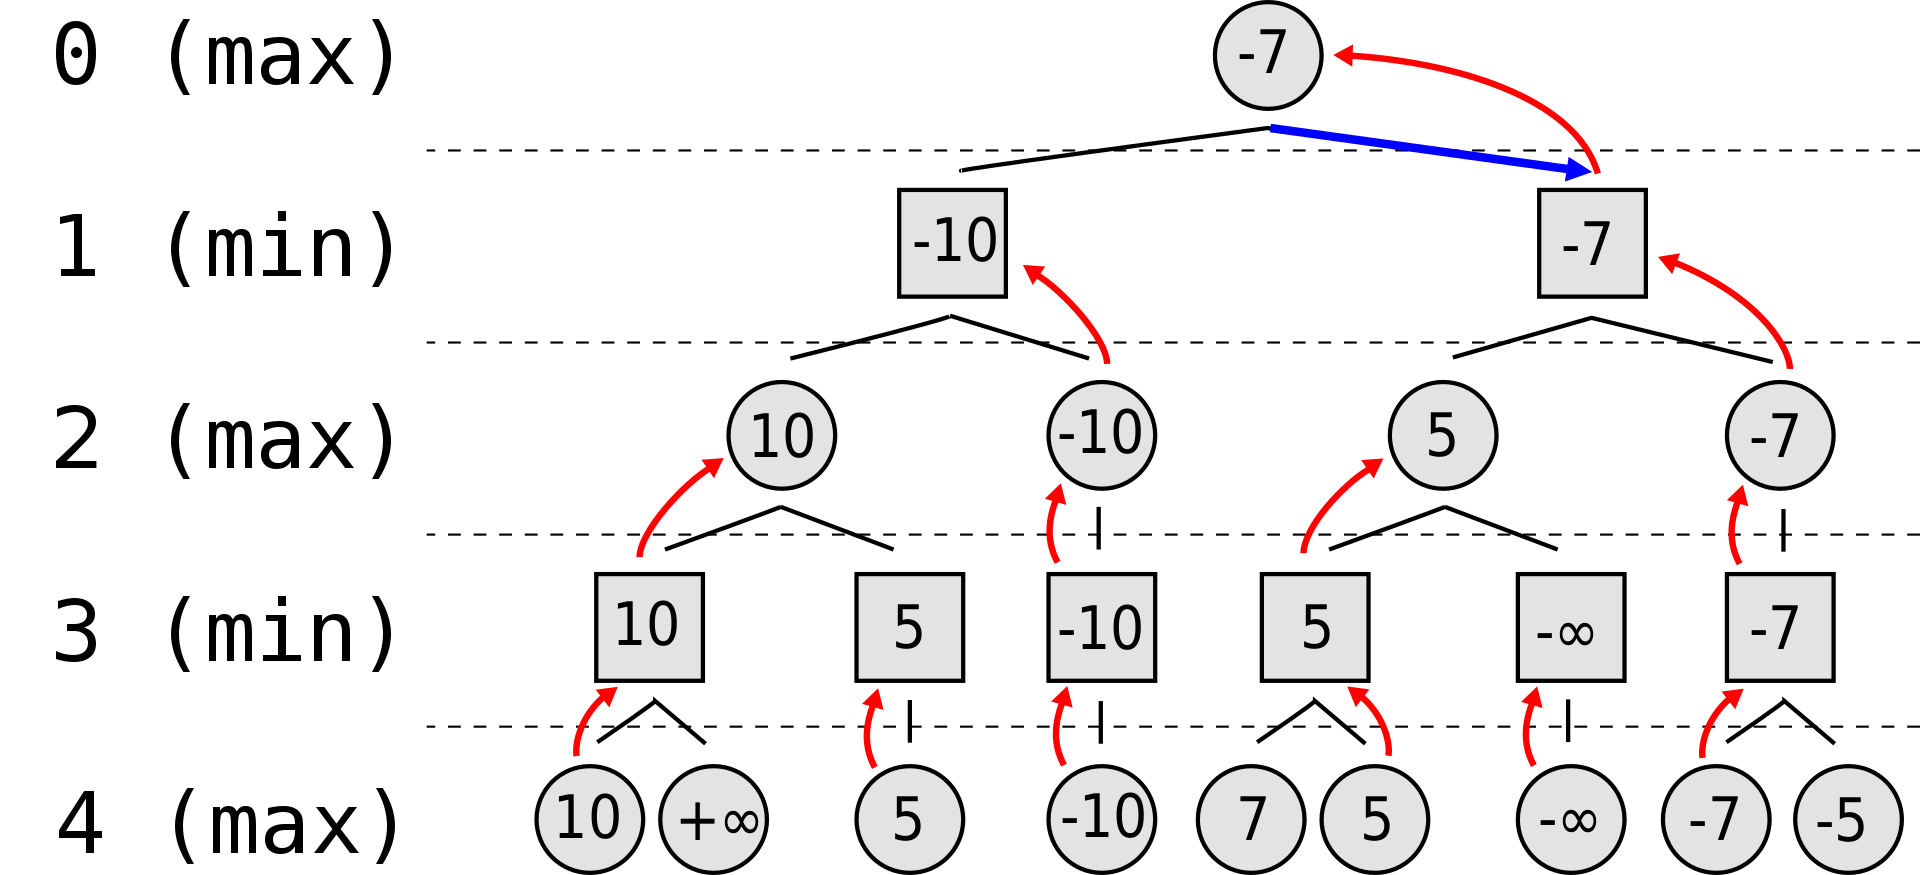
\includegraphics[width=\textwidth]{1920px-Minimax.svg.png}\\
    \label{fig:Tree Example}
\end{figure}

The Minimax tree shows an example of how the minimax works. In this scenario the maximizer goes first, and has 2 possible moves. 
The maximizer would therefore explore the first move first, marked -10. At this point the algorithm has not simulated this move yet and therefore does not know that value yet. 
So first it just tries the moves leftmost in the tree until it hits the depth 4 which is the bottom in this scenario. It would end up with a value of 10 which would be good for the maximizer. 
However, the minimizer needs to be taken into account, so the maximizer backtracks once to see the other move which is +infinity. 
It is guaranteed, that the minimizer would never pick that route, which means the score 10 can be kept in mind while the maximizer backtracks to the next point where the minimizer has a move. 
As is seen this route only gives both players one choice on each of their respective turns. 
The last move has a -10 score so it backtracks with that score once again and ends up with 10 and -10 on the 2 moves the minimizer can make. 
If the maximizer chooses this route the point value of the move would therefore be -10 as the minimizer always goes for the lesser score.\\
The algorithm then does the same thing for the other branch of moves and finds that this move will serve the maximizer better as it will yield -7 move value which is still poor for the maximizer but less so than a -10 score.

\subsection{Implementation of Minimax}
\label{subsec:Implementation of Minimax}
% Show our own code!
\begin{lstlisting}[language=python, caption={python example}, label={Script}, basicstyle=\ttfamily\small]
    # AI makes a move based on minmax algorithmic search for the most rational move to make
    def ai_move(board):
        best_move = board
        best_value = float('-inf')
        for move in all_possible_moves(board, AI):
            #print(move)
            move_val = minimax(move, 0, False)
            #print(move_val)
            if move_val > best_value or best_value == None:
                best_move = move
                best_value = move_val
        return best_move
\end{lstlisting}

The function ai\textunderscore move gets called when its the AI's turn to play. The function generates a list of all possible moves from the current board, 
which the function recieves from the arguments.
This list is then iterated over to run the minimax recursion on each of these possible moves.
When the result move\textunderscore val is received for the current move, this value is then checked to see if it is higher or equal to the stored best\textunderscore value. 
If it is, that stored value is then overridden with the new best value.

\begin{lstlisting}[language=python, caption={python example}, label={Script}, basicstyle=\ttfamily\small]
    def minimax(board, depth, isMax):
    score = evaluate(board)
    
    if score == 10: 
        return score
    if score == -10:
        return score
    if board.count(EMPTY) == 0:
        return 0

    if isMax:
        best = float('-inf')
        for move in all_possible_moves(board, AI):
            best = max(best, minimax(move, depth + 1, not isMax))
        return best
    else:
        best = float('inf')
        for move in all_possible_moves(board, HUMAN):
            best = min(best, minimax(move, depth + 1, not isMax))
        return best
\end{lstlisting}

This is the implementation made in Simon's Original Jupyter Notebook. 
The function always starts by checking the board with another function called evaluate. 
This function checks for win conditions and returns either 10 if the AI has a winning board and likewise -10 for the Human player.
If no one has won yet it returns 0.

Next the received score is checked to find out if the recursion for this move should end. This is done if the score is -10, 10 or 0, 
and as expected the move will not be considered as best 
if the score is -10 as the AI does not want the human player to win.

The next part of the implementation is the interesting part. First the current simulated move is checked to see if it is the maximizer's (Human) or the minimizer's (AI) turn. 
Depending on the result of this the recursion is set up oppositely. A "best" variable is started at the worst value for the player being 
-infinity for the maximizer and infinity for the minimizer. This is done to ensure that there is a value to overwrite on the very first run of the algorithm.
A list of possible moves is then created for this current simulated board and iterated over. This is where the recursion happens.
The minimax function is called within it self on the current considered move of the list. This ensures that all possible moves are evaluated for this new current board as well, 
because every time the function returns "best" it backtracks to check the next move. Remember the tree example explained in figure~\ref{fig:Tree Example}.
\clearpage

\section{Alpha/Beta Pruning} 
\label{sec:Alpha/Beta Pruning}

\subsection{Introduction to Alpha/Beta Pruning}
\label{subsec:Introduction to Alpha/Beta Pruning}
Alpha/Beta pruning is a way by which the Minimax Algorithm is made more efficient.
This happens by stopping consideration of possible moves, that will never be better than previously considered moves.

\subsection{Explanation of Alpha/Beta Pruning}
\label{subsec:Explanation of Alpha/Beta Pruning}
Alpha Beta Pruning is an optimization method for the Minimax algorithm that eliminates branches or entire subtrees. 
It is so named because it introduces the two variables or values Alpha and Beta into the Minimax algorithm.
According to Akshay L Aradhya who wrote \href{https://www.geeksforgeeks.org/minimax-algorithm-in-game-theory-set-4-alpha-beta-pruning/}{this article}:
"Alpha is the best value that the maximizer currently can guarantee at that level or above.
Beta is the best value that the minimizer currently can guarantee at that level or above."
\begin{figure}
    \centering % Centering requirement met
    \begin{subfigure}[b]{0.3\textwidth}
        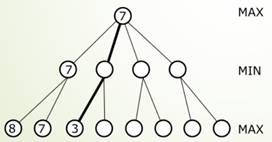
\includegraphics[width=\textwidth]{AlphaBetaPruning1.png}           
    \end{subfigure}
    ~
    \begin{subfigure}[b]{0.3\textwidth}
        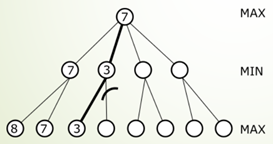
\includegraphics[width=\textwidth]{AlphaBetaPruning2.png}       
    \end{subfigure}
    \caption{An example of Alpha Beta Pruning.} % Caption beneath both of the images.
    \label{fig:AlphaBetaPruningA}
  \end{figure}
Figure \ref{fig:AlphaBetaPruningA}  shows how first the leftmost branches are explored 
and the minimizer picks “7” which is stored in the variable Alpha. 
After that the second leftmost branch is explored and the Minimizer is presented with a choice that is smaller than 7.
Given that there is a choice smaller than Alpha present already, and it is the Minimizer’s turn to choose, 
meaning that it will undoubtedly have a chance to pick a value smaller than Alpha, 
it would not be worth it for the Maximizer to explore the rest of the branch and the branch is pruned as seen 
in figure \ref{fig:AlphaBetaPruningA}.
\begin{figure}[!t]
    \centering % Centering requirement met
    \begin{subfigure}[t]{0.3\textwidth}
        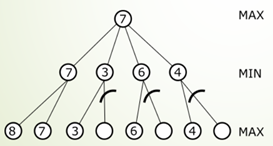
\includegraphics[width=\textwidth]{AlphaBetaPruning3.png}
    \end{subfigure}
    ~
    \begin{subfigure}[t]{0.3\textwidth}
        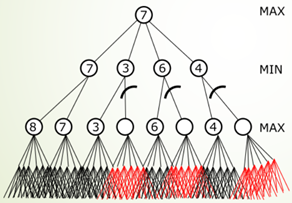
\includegraphics[width=\textwidth]{AlphaBetaPruning4.png}
    \end{subfigure}
    \caption{An example of many branches being pruned.} % Caption beneath both of the images.
    \label{fig:AlphaBetaPruningB}
  \end{figure}
Alpha Beta Pruning can potentially prune a lot of branches and 
thus make the examination of choices or moves through Minimax considerably faster 
than if it simply went through every single branch as seen in figure~\ref{fig:AlphaBetaPruningB}.
\subsection{Implementation of Alpha/Beta Pruning}
\label{subsec:Implementation of Alpha/Beta Pruning}
This section shows the changes to the minimax function and more, which was added to version 3 of the notebook in the code folder. This was done to better see the results of the pruning. 
First thing that was done was to add a counter to the minimax function in both version 3 and 4 of the code. This counter increments every time a new future move is considered. 
The idea was to show a count of how many moves the AI had considered before making the most rational choice. This way the number of considered moves on both versions of the code could be compared:
one before implementing pruning and one after.
\begin{lstlisting}[language=python, caption={python example}, label={Script}, basicstyle=\ttfamily\small]
    def minimax(board, depth, alpha, beta, isMax):
        global count 
        score = evaluate(board)
        count += 1
        if score == 10: 
            return score
        if score == -10:
            return score
        if board.count(EMPTY) == 0:
            return 0
        
        if isMax:
            maxEval = float('-inf')
            for move in all_possible_moves(board, AI):
                evaluation = minimax(move, depth + 1, alpha, beta, not isMax)
                maxEval = max(maxEval, evaluation)
                alpha = max(alpha, evaluation)
                if beta <= alpha:
                    break
            return maxEval
        else:
            minEval = float('inf')
            for move in all_possible_moves(board, HUMAN):
                evaluation = minimax(move, depth + 1, alpha, beta, not isMax)
                minEval = min(minEval, evaluation)
                beta = min(beta, evaluation)
                if beta <= alpha:
                    break
            return minEval
\end{lstlisting}
To implement Alpha Beta Pruning 2 more parameters had to be added to the function: alpha and beta. These start with the values -infinity and infinity.
The recursive call was then updated to have these arguments included. For the maximizer the alpha value was set to whichever is greater between the current alpha value and the evaluation.
Likewise it is done for the minimizer between which is lesser of beta's current value and the evaluation. This means that every time the minimax function is run, the alpha value is updated if it is the maximizing players turn. 
Likewise the beta value is updated on the minimizing players turn.
No matter whose turn it is beta is checked to see if is less than or equal to alpha, and if this is true, the rest of the moves are pruned.
\clearpage

\section{Discussion} 
\label{sec:Discussion}

\subsection{Compare results}
This subsection will be used to show the results of the pruning.\\
In the notebook without pruning (V3) on turn 1 the AI considered 549945 different moves.
In the notebook with pruning (V4) on turn 1 the AI considered 30709 different moves.\\
This means that on turn one V4 managed to prune away around 93\% of the moves that would be considered without pruning.\\
On turn 3 this went from 7331 down to 1519 which is again a significant decrease of around 80\%.
These prunings of course become smaller in number as the game had fewer possible moves, and at turn 7 it would no longer prune anything.\\
These findings can be seen better by running files \href{code/TicTacToe_MinimaxV3.ipynb}{MinimaxV3.ipynb} 
and \href{code/TicTacToe_MinimaxV4.ipynb}{MinimaxV4.ipynb} in the code folder of this project.

%\subsection{Reflection}
\subsection{Conclusion}
%Brief summary:What  has  been  done  and  the  benefits  of  it. Recommendation for future extensions and upgrades. Reflection on the work and the product.
The Jupyter Notebook TicTacToe\textunderscore MinimaxV4.ipynb is the result of the implementation of 
Alpha Beta Pruning that was compared with the original notebook.
Version 4 has significantly fewer considered moves, presumably resulting in a slightly faster game 
for this implementation of Tic-Tac-Toe.
If implemented on a game like chess, which requires the algorithm to check many more moves per depth, 
pruning would likely save an considerable amount of time compared to the bare minimax function.\\
Future implementations, that would be interesting to include, could be: input validation, Multiplayer (humans), AI versus AI games, allowing for picking X or O, 
a choice of board size and potentially different games. Of those it would be relevant to test Alpha Beta Pruning on future versions 
with allowing for picking X or O and on different board sizes.\\
% Reflection: what went well, what could be better
For a small project like this, simply comparing the amount of considered moves between notebook versions has worked well.
On the other hand, more precise tools could have been used to compare and to test efficiency and impact of Alpha Beta Pruning.

\begin{thebibliography}{1}
    \label{thebibliography}

    \bibitem{Tic-Tac-ToeBoard}
    \label{bib:Tic-Tac-ToeBoard}
    Danforth Pewter.\\
    \textit{Tic Tac Toe Board w/Pouch}, \url{https://www.danforthpewter.com/wooden-tic-tac-toe-board.html}\\
    Webshop selling a wooden Tic-Tac-Toe board.

    \bibitem{MinimaxTreeExample}
    \label{bib:MinimaxTreeExample}
    Nuno Nogueira.\\
    \textit{A minimax tree example}, \url{https://en.wikipedia.org/wiki/Minimax#/media/File:Minimax.svgl}\\
    Image for Wikipedia Article on Minimax.

    \bibitem{MinimaxVideo}
    \label{bib:MinimaxVideo}
    Sebastian Lague, Game Developer and Online Tutor.\\
    \textit{Algorithms Explained – minimax and alpha-beta pruning}, \url{https://www.youtube.com/watch?v=l-hh51ncgDI}\\
    From his tutorial channel on Youtube.\\
    Credibility: Sebastian Lague's video on minimax and alpha beta pruning is viewed as credible, because it was added as a link on the Data Science Courses materials on week 7.
    \url{https://datsoftlyngby.github.io/soft2021spring/DSC/week-07/#6-introduction-to-data-science-and-development-environment}\\


    \bibitem{AlphaBetaSlides}
    \label{bib:AlphaBetaSlides}
    Martin Vestergaard (mrv@cphbusiness.dk), Todorka Dimitrova (tdi@cphbusiness.dk)\\
    \textit{Data Science}, \url{https://datsoftlyngby.github.io/soft2021spring/resources/46f5e513-01-intro-and-minimax.pdf#page=100}\\
    From the Data Science lecture PowerPoint Presentation "Data Science" slides from week 7 on pages 100 to 104.

    \bibitem{MinimaxAlphaBetaArticle}
    \label{bib:MinimaxAlphaBetaArticle}
    Akshay L Aradhya.\\
    \textit{Minimax Algorithm in Game Theory | Set 4 (Alpha-Beta Pruning)}, \url{https://www.geeksforgeeks.org/minimax-algorithm-in-game-theory-set-4-alpha-beta-pruning/}\\
    From the tutorial/guide website GeeksForGeeks.org.

    \bibitem{OurCode}
    \label{bib:OurCode}
    Simon Schønberg Bojesen, Frederik Blem.\\
    \textit{UFO\textunderscore Exam\textunderscore Minimax\textunderscore Paper/code/}, \url{https://github.com/FrederikBlem/UFO_Exam_Minimax_Paper/tree/main/code}\\
    This is the code folder of our Github Repository.

    
        % \bibitem{FirstBook} 
        % Author A, Author B and Author C. 
        % \textit{The First Book Name}. 
        % Publisher 1, Reading, City Name, Year.
        
        % \bibitem{How to get a paper accepted at oopsla} 
        % Kent Beck. 
        % \textit{How to get a paper accepted at oopsla, 1993}
        
        % \bibitem{Studieordning} 
        % Copenhagen Business Academy.\\
        % \textit{Studieordning  for  professionsbacheloruddannelsen  i  soft-wareudvikling}. (Danish) 
        % [\textit{Curriculum forthe Bachelor’s Degree Programme in Software Development, aug 2017}].
        % \\\url{https://datsoftlyngby.github.io/soft2020fall/resources/bbe51cf2-bachelorProject.pdf}
        
\end{thebibliography}

\end{document}